\documentclass[margin,letterpaper,11pt]{scrartcl}
\usepackage[latin1]{inputenc}
\usepackage{alltt}
\usepackage{enumerate}
\usepackage[normalem]{ulem}
\usepackage[english]{babel}
\usepackage{graphicx}
\usepackage{epstopdf}
\usepackage{listings}
\setlength{\textwidth}{6.5in}
\setlength{\textheight}{9in}
\setlength{\oddsidemargin}{0in}
\setlength{\evensidemargin}{\oddsidemargin}
\setlength{\topmargin}{0in}
\setlength{\headsep}{0in}
\setlength{\headheight}{0in}
\setlength{\parindent}{0in}
\parskip 7.2pt

% figure width
\newlength \figwidth
\setlength \figwidth {0.8\textwidth}
% figure half width
\newlength \fighwidth
\setlength \fighwidth {0.4\textwidth}

\begin{document}

% paper size
\special{papersize=8.5in,11in}
\setlength{\pdfpageheight}{\paperheight}
\setlength{\pdfpagewidth}{\paperwidth}

\title{Mushroom Analysis Writeup}
\subtitle{CSCI 568 - Data Mining}
\date{21 November, 2011}
\author{Brandon Vargo}
\maketitle

\section{Getting started}

I started the project by reading the metadata file (mushroom.meta.txt), in
order to get a feeling for the data contained within the dataset, such as the
attribute types. I found that the data describes a number of attributes about
mushrooms, and the primary ``objective'' of the dataset is determining whether
a given mushroom is poisonous. If the edibility status is unknown, then a
mushroom is classified as poisonous.

Next, I looked at the data file itself (mushroom.data.csv). In particular, I
looked at the format of the data and for any missing attributes. I found that
the data was a standard CSV file with no missing attributes, matching the
information found in the metadata file. The first attribute is the edibility
of the mushroom, and the other attributes correspond to the attributes listed
in the metadata file.

For this assignment, I decided to continue using Weka. So far, Weka has proved
easier to use than Knime, and I have not had a need to switch to Knime yet. For
the purposes of filtering data, I used gnumeric, an Excel-like clone, in order
to browse and filter the data as needed. I also tried Weka's filtering,
particularly the RemoveUseless unsupervised instance filter, but it was not
particularly effective.

\section{Can you generate summary statistics that help describe the data?}

All of the twenty-two attributes are nominally valued. That is, each attribute
has a finite number of discrete values that are assigned in name. This makes
it difficult to generate summary statistics, such as averages. It does not
make sense to ask the average of bell, conical, convex, flat, knobbed, and
sunken for the shape of the mushroom cap.

That said, it is possible to look at the distribute of nominal labels among
particular groups. Figure~\ref{fig:summary_stat} shows the distribution of edible
vs poisonous among all of the attributes. This view allows an analyst to
easily look at the data from a ten-thousand foot view. In this case, we can
see that some attribute values are evenly distributed, while other attribute
values are extremely rare. For example, the cap shape of c (convex) is rare,
with only 4 mushroom data points having convex cap shapes, while all of the
mushrooms have the veil type of p (partial). There does not appear to be a
single attribute that can identify edible mushrooms, though odor appears to
come close if the odor values are grouped.

\begin{figure}[!htb]
\begin{center}
   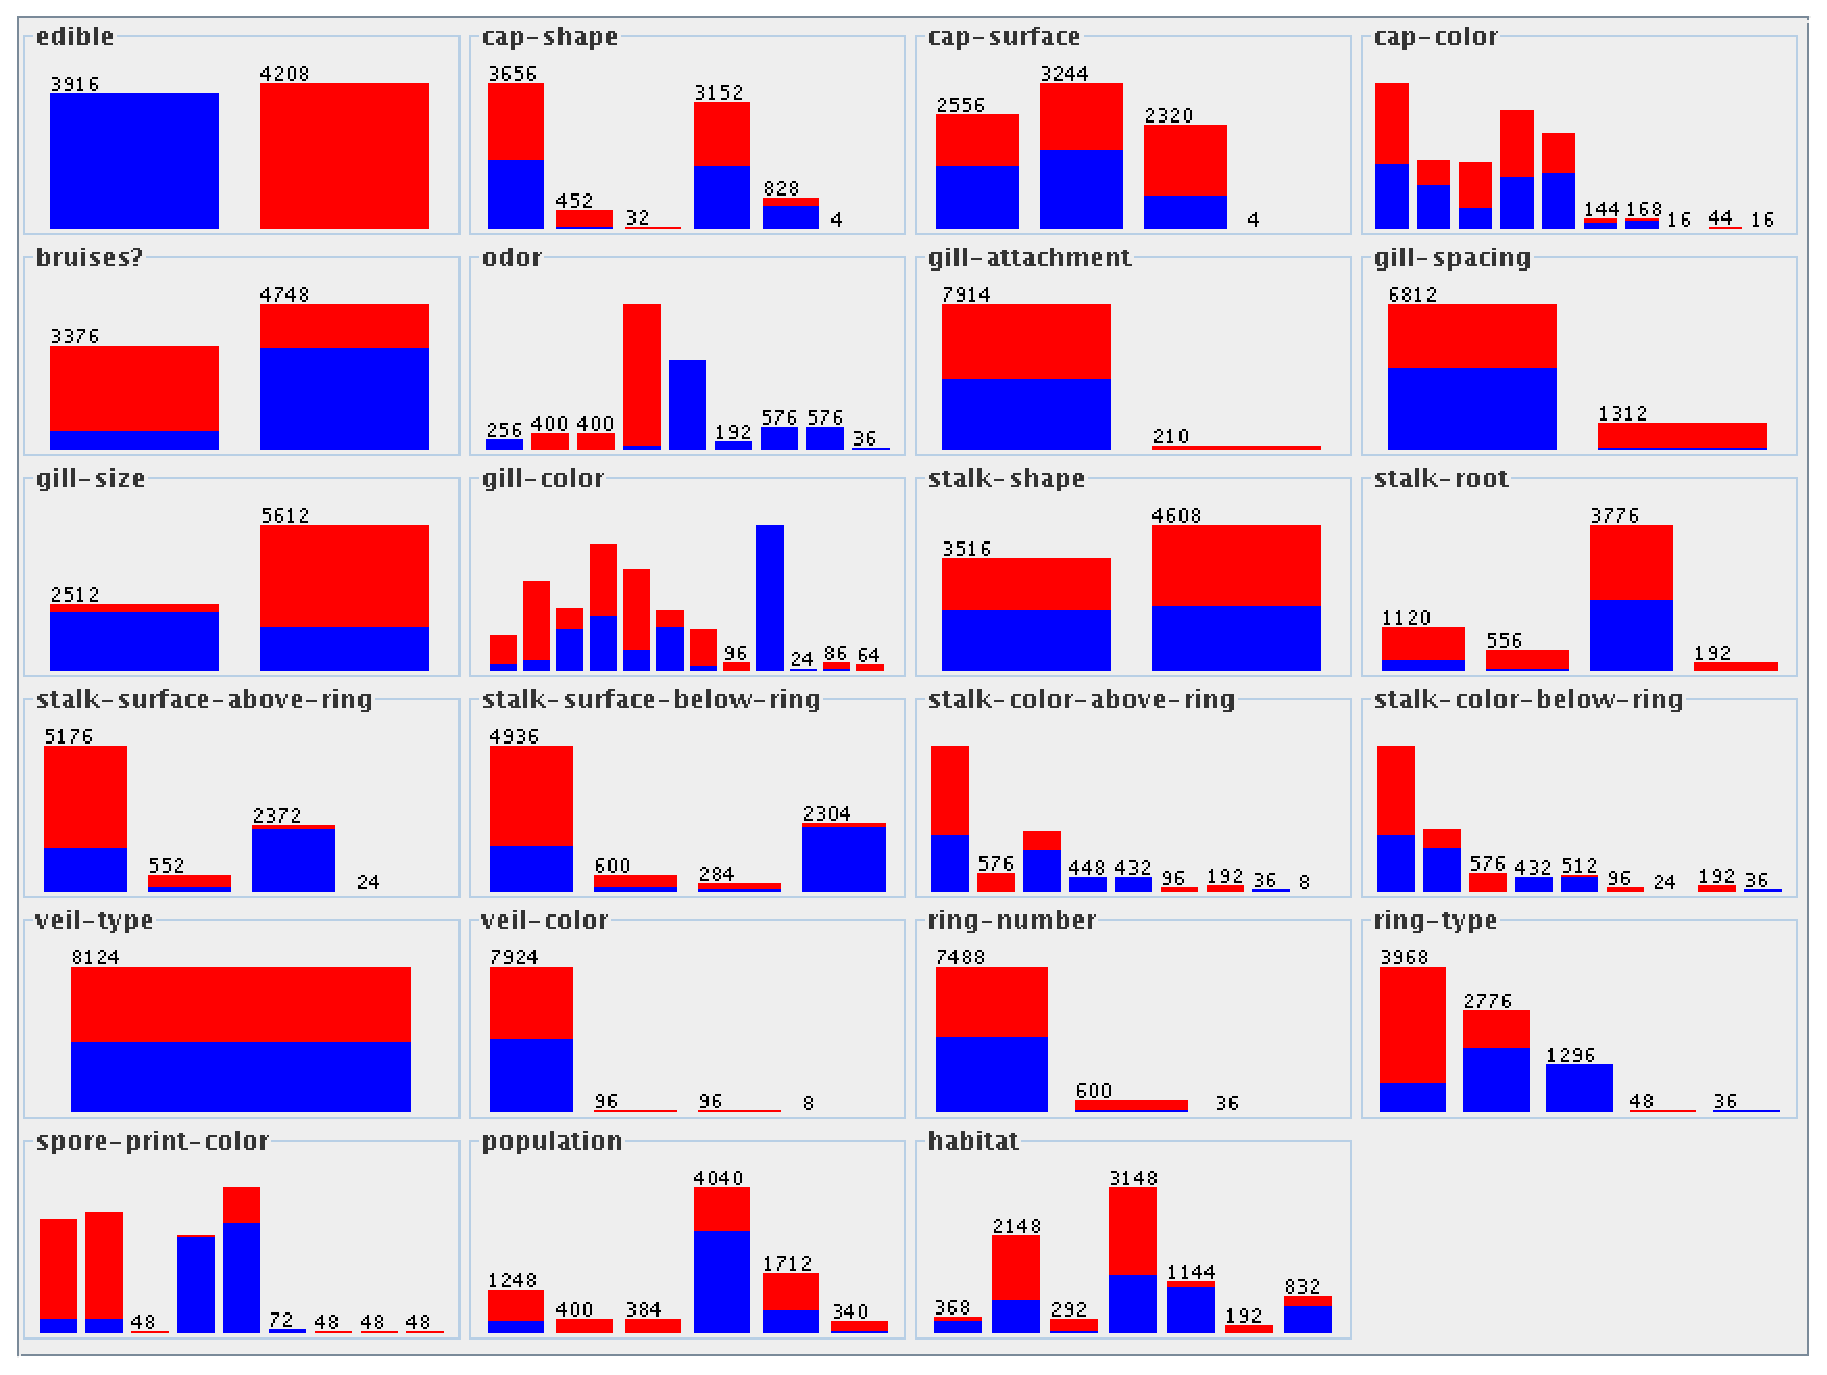
\includegraphics[width=\figwidth]{images/summary.eps}
   \caption{The distribution of edibility among the class attributes. Blue is
   poisonous, while red is edible.}
   \label{fig:summary_stat}
\end{center}
\end{figure}

\section{Can the edible and poisonous data objects be distilled into groups?}

Upon initial glance, not easily. As noted above, odor appears to come close.
If the odors N, L, and A (non, anise, and almond) are combined as one group,
and all other odors are another group, then few mushrooms are misclassified.
How many is a few? Weka, the tool that produced the above analysis, does not
have an easy mechanism to show how many records are a given color within a
single bar. Using other tools, it can be shown that 120 mushrooms are
misclassified using this method, as there are 120 poisonous mushrooms with no
odor. This represents an error rate of just under 1.5\%. This is not bad for
looking at a few colors on the screen!

Taking a more scientific group, I decided to try clustering, seeing ``groups''
in the question. However, since the attributes are nominal, then clustering
probably does not make much sense. There is not a good metric for defining the
distance between two objects. Nevertheless, I gave the data to Weka's EM
clustering algorithm. It ran for quite some time before I ended the process,
knowing that the results would probably not be very useful given the nominal
attributes.

\section{Can a classification model be created that can predict whether a
mushroom is edible or poisonous?}

\subsection{Tree-based classifier}

To answer this question, I initially used Weka's SimpleCart algorithm, a
tree-based classifier. It produced the following tree:

\begin{alltt}
odor=(a)|(l)|(n)
|  spore-print-color=(k)|(n)|(u)|(h)|(o)|(y)|(b)|(w)
|  |  stalk-color-below-ring=(p)|(g)|(e)|(o)|(w)|(n)|(b)|(c)
|  |  |  cap-surface=(s)|(f)|(y)
|  |  |  |  stalk-color-below-ring=(p)|(g)|(e)|(o)|(w)|(b)|(y)|(c): e(4144.0/4.0)
|  |  |  |  stalk-color-below-ring!=(p)|(g)|(e)|(o)|(w)|(b)|(y)|(c)
|  |  |  |  |  stalk-surface-above-ring=(s)|(f)|(y): e(64.0/0.0)
|  |  |  |  |  stalk-surface-above-ring!=(s)|(f)|(y): p(16.0/0.0)
|  |  |  cap-surface!=(s)|(f)|(y): p(4.0/0.0)
|  |  stalk-color-below-ring!=(p)|(g)|(e)|(o)|(w)|(n)|(b)|(c): p(24.0/0.0)
|  spore-print-color!=(k)|(n)|(u)|(h)|(o)|(y)|(b)|(w): p(72.0/0.0)
odor!=(a)|(l)|(n): p(3796.0/0.0)
\end{alltt}

Note that the first decision made is whether the odor should is one of a, l,
or n. This is the same classification model that was identified above by
looking at the summary diagram. The rest of the decision tree generated
reduces the error to five mushroom instances, or 0.0615\% of the records.

In some of the nodes above, the support of the path to the node is very low.
For example, the \texttt{cap-surface!=(s)|(f)|(y)} decision only affects four
records, while the remaining records ``travel down'' the other side of the
branch. This may be a case of overfitting, as these records may be anomalies,
or they may be legitimate mushrooms.

\subsection{Rule-based classifier}

Weka's PART classifier, a rule classifier, produces the following thirteen
rules. This ruleset correctly identifies whether a mushroom can be eaten in
all cases for the data.

\begin{alltt}
odor = f: p (2160.0)
gill-size = b AND ring-number = o: e (3392.0)
ring-number = t AND spore-print-color = w: e (528.0)
odor = y: p (576.0)
odor = s: p (576.0)
stalk-shape = e AND stalk-surface-below-ring = s AND odor = p: p (256.0)
stalk-shape = e AND odor = c: p (192.0)
gill-size = n AND stalk-surface-above-ring = s AND population = v: e (192.0)
gill-size = b: p (108.0)
stalk-surface-below-ring = s AND bruises? = f: e (60.0)
stalk-surface-below-ring = y: p (40.0)
bruises? = f: e (36.0)
: p (8.0)
\end{alltt}

See the anomaly section below for a short discussion on these rules, and why
more knowledge is needed to determine whether this model is overfitting the
data or whether the rules could match a larger set of mushrooms effectively.

\section{Do any anomalies exist in the dataset?}

Maybe. There are certainly small groups of mushrooms that do not match rules that
cover most of the dataset, as outlined below. Whether these small groups of
mushrooms can be considered outliers, or whether these mushrooms happen to be
part of another group that is not included in the dataset is specific to the
domain. With respect to the dataset, these mushrooms may be outliers.

Applying a traditional statistical approach is not easy in this application,
due to the large number of dimensions, all of which are nominal attributes.
Thus, it makes more sense to produce a model and look at the cases that the
model does not match the data. The data may be ``wrong'' in the sense that the
non-matching records are outliers. Likewise, the model could be ``wrong'' in
the sense that it does not encompass all of the complexities of mushrooms,
either due to not enough data records or hidden attributes that could not be
included in the model. For example, in the above approach of looking at the
Weka colored output, are the 120 misclassified mushrooms outliers? Perhaps.
What about the 8 mushrooms that final rule of the rule-based classifier
matches? Perhaps. More evaluation is necessary, with more domain-specific
knowledge.

\section{Can any association rules be generated from this dataset?}

Once again, I used Weka in order to answer this question. Using the apriori
association algorithm with a minimum support of 0.95 and a minimum confidence
of 0.9, the following are the top ten rules generated by Weka:
\begin{alltt}
 1. veil-color=w 7924 ==> veil-type=p 7924    conf:(1)
 2. gill-attachment=f 7914 ==> veil-type=p 7914    conf:(1)
 3. gill-attachment=f veil-color=w 7906 ==> veil-type=p 7906    conf:(1)
 4. gill-attachment=f 7914 ==> veil-color=w 7906    conf:(1)
 5. gill-attachment=f veil-type=p 7914 ==> veil-color=w 7906    conf:(1)
 6. gill-attachment=f 7914 ==> veil-type=p veil-color=w 7906    conf:(1)
 7. veil-color=w 7924 ==> gill-attachment=f 7906    conf:(1)
 8. veil-type=p veil-color=w 7924 ==> gill-attachment=f 7906    conf:(1)
 9. veil-color=w 7924 ==> gill-attachment=f veil-type=p 7906    conf:(1)
10. veil-type=p 8124 ==> veil-color=w 7924    conf:(0.98)
\end{alltt}

All of the results that have a consequent of only veil-type are worthless. All
of the data has a veil-type of p, so of course any antecedent is going to
produce a consequent with a veil-type of p!

After running the generator again, this time ignoring veil-type, the following
rules are produced:
\begin{alltt}
 1. veil-color=w ring-number=o 7288 ==> gill-attachment=f 7288    conf:(1)
 2. gill-attachment=f gill-spacing=c 6602 ==> veil-color=w 6602    conf:(1)
 3. gill-spacing=c veil-color=w ring-number=o 6272 ==> gill-attachment=f 6272    conf:(1)
 4. gill-attachment=f gill-spacing=c ring-number=o 6272 ==> veil-color=w 6272    conf:(1)
 5. gill-attachment=f gill-size=b 5402 ==> veil-color=w 5402    conf:(1)
 6. stalk-surface-above-ring=s veil-color=w 4984 ==> gill-attachment=f 4984    conf:(1)
 7. gill-attachment=f stalk-surface-above-ring=s 4984 ==> veil-color=w 4984    conf:(1)
 8. gill-size=b veil-color=w ring-number=o 4784 ==> gill-attachment=f 4784    conf:(1)
 9. gill-attachment=f gill-size=b ring-number=o 4784 ==> veil-color=w 4784    conf:(1)
10. stalk-surface-below-ring=s veil-color=w 4744 ==> gill-attachment=f 4744    conf:(1)
\end{alltt}

Again, most of these rules are pointless. In order to try and find more
interesting associations, let us remove all attributes that are predominantly
dominated by a single value: gill-attachment, gill-spacing, veil-type,
veil-color, and ring-number. The following rules are produced:
\begin{alltt}
 1. odor=n gill-size=b 3288 ==> edible=e 3216    conf:(0.98)
 2. bruises?=t stalk-surface-below-ring=s 3040 ==>
      stalk-surface-above-ring=s 2968 conf:(0.98)
 3. odor=n 3528 ==> edible=e 3408    conf:(0.97)
 4. stalk-surface-below-ring=s ring-type=p 3472 ==>
      stalk-surface-above-ring=s 3328 conf:(0.96)
 5. bruises?=t 3376 ==> stalk-surface-above-ring=s 3232    conf:(0.96)
 6. bruises?=t ring-type=p 3184 ==> stalk-surface-above-ring=s 3040    conf:(0.95)
 7. gill-size=b stalk-surface-above-ring=s stalk-surface-below-ring=s 3064 ==> 
      edible=e 2920    conf:(0.95)
 8. bruises?=t gill-size=b 3016 ==> stalk-surface-above-ring=s 2872    conf:(0.95)
 9. edible=e ring-type=p 3152 ==> stalk-surface-above-ring=s 2992    conf:(0.95)
10. edible=e odor=n 3408 ==> gill-size=b 3216    conf:(0.94)
\end{alltt}

These rules may be considered more useful. However, I am not a mushroom expert,
so more domain knowledge is needed in order to determine the qualitative
quality of the rules.

\end{document}
